% !TeX program = PdfLaTeX
% !TeX root = ../../Elaborati_Aerodinamica_Bruno_Spoti.tex

\chapter{Introduzione}
In questa terza parte ci si prefigge di caratterizzare l’aerodinamica del velivolo di linea quadrimotore \emph{Airbus A340-200}. \cite{author:airbusA340}.\\
%Preliminarmente sono stati reperiti i dati di principale interesse.
\begin {figure} [h!]
\centering
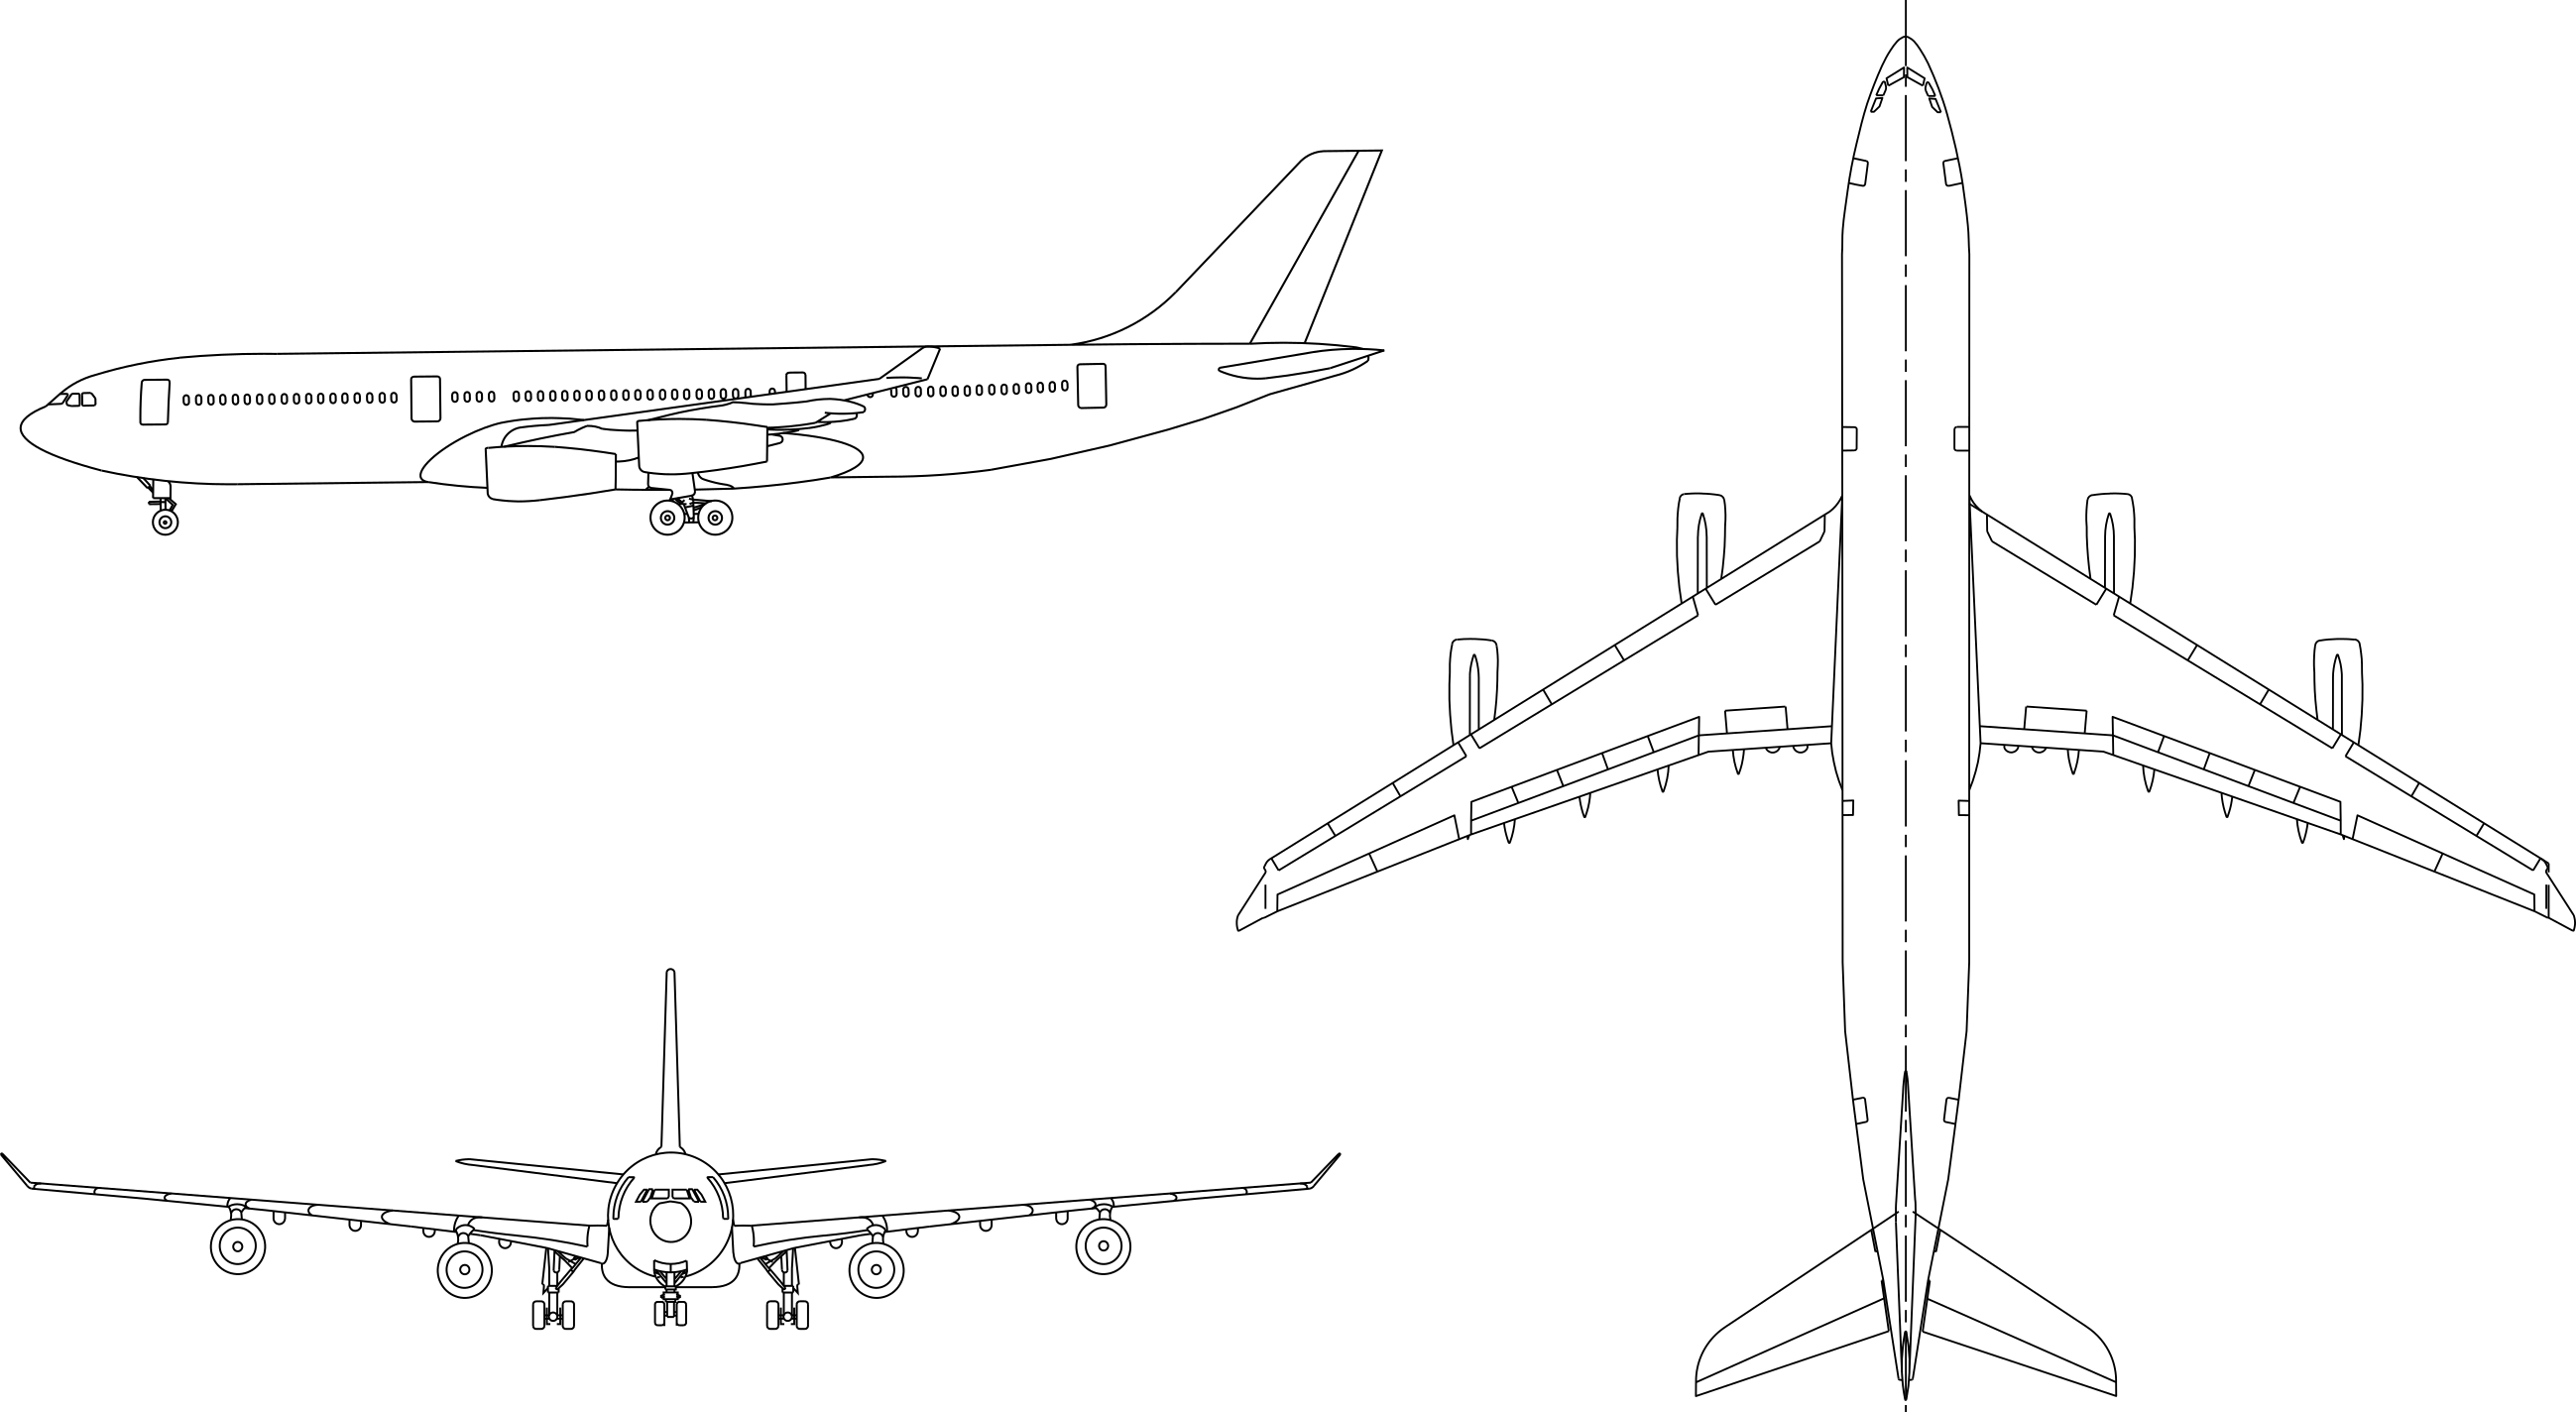
\includegraphics[width= \textwidth ]{images/fileImg/Parte_3-Aerodinamica_Velivolo_A340-200/tritticoA340-200.png}
\caption{\footnotesize Trittico Airbus A340-200}
\label {fig:trittico}
\end {figure}

Nella tabella~\ref{tabV1} e~\vref{tabV2}  sono elencanti i dati geometrici d'interesse del velivolo. \cite{author:airbusA340} \cite{author:Jane}  \\ \\ 


\begin{table} [!h]\centering \rowcolors{1}{}{grigio_chiaro}
\begin{tabular}{l c c}
\toprule
\multicolumn{3}{c}{\emph{Dati Geometrici}} \\ 
\midrule
Apertura Alare 		& $b$  					&   	$60.30 \si{m} $ 		\\
Superficie Alare & $S_\mathrm{w}$  		&  		$361.6 \si{m^2} $ 		\\
Allungamento alare & $\AR$ 				& 	    $10.56$ 				\\
Corda alla radice & \croot	&  	$10.6 \si{m}$   \\
Corda all'estremità & \ct							&  		$2.57 \si{m}$ 	    \\
Corda alla sezione di \emph{kink} & \ck							&  		$7.20 \si{m}$ 	    \\
%Fattore di Oswald & $e$	   				& 	    $0.75 $ 				\\
Angolo di freccia al bordo d'attacco & $\Lambda_{le}$ & $32.2^\circ $  \\ 
Angolo diedro dell'ala  & $\Gamma_\mathrm{W}$ & $4.56^\circ $ \\
\midrule
Lunghezza totale  & $L$  					&   	$59.42 \si{m} $ 		\\
Altezza totale & $H$  					&   	$16.84 \si{m} $ 		\\
Massimo diametro della fusoliera & \Dfmax  					&   	$5.64 \si{m} $ \\
Apertura piano di coda orizzontale  &\bHtail & $ 19.41\si{m} $		\\ 

	
\bottomrule
\end{tabular}
\caption {\footnotesize Dati geometrici principali del velivolo Airbus A340-200}
\label{tabV1}
\end{table}

\begin{table} [!h]\centering \rowcolors{1}{}{grigio_chiaro}
	\begin{tabular}{l c c}
		\toprule
		\multicolumn{3}{c}{\emph{Pesi e prestazioni}} \\ 
		\midrule
		Peso a vuoto operativo (OWE) & \WOE & 129500 \si{kg} \\
		Massimo carico pagante & \WPLmax & 45530 \si{kg} \\
		Peso massimo al decollo configurazione base (MTOW)   &\MTOW & 253500 \si{kg} \\
		Peso massimo al'atterraggio    &\WLmax & 181000 \si{kg} \\
		Peso massimo senza carburante    &\Wzfmax & 169000 \si{kg} \\
		Carico alare massimo   &\WoverSmax & 760.5 \si{kg/m^2} \\
		\midrule		
		Numero di Mach massimo operativo & \Mmo & 0.86 \\
		Velocità massima operativa (IAS)  & \Vmo 	&  	$661 \si{km/h} $ 	\\
		Mach di crociera & \Mc &  	$0.82 $ 	\\
		Velocità di crociera & \Vc &  	$630 \si{km/h}$ 	\\
		Velocità di stallo {\itshape full flap} (267000kg, \emph{wheels up})	 & \Vsf 	&  	$247 \si{km/h} $  	\\
		Velocità di stallo {\itshape clean configuration}   & \Vsc&  $299 \si{km/h} $	\\
    	Quota massima certificata & \hmax & 12525 \si{m}\\
		Distanza di decollo	(S/L, MTOW, ISA +15°C) &	\TOFL & 3017 \si{meter}  \\
		Autonimia di distanza con 239 passeggeri &	$R$ & 14816 \si{km}  \\
		\bottomrule
\end{tabular}
	\caption {\footnotesize Pesi e prestazioni caratteristiche del velivolo Airbus A340-200}
	\label{tabV2}
\end{table}

%\begin{table} [!h]
%
%\centering
%\begin {tabular} {lp{6cm} l}
%{\bfseries Dato }  & & { \bfseries Valore} \\ 
%\hline \hline
%Velocità di crociera {\bfseries $V_c$}  & &  $59.16 m/s $ \\
%\hline
%Velocità massima {\bfseries $V_{max}$}  & &   $64.30 m/s $ \\
%\hline
%Velocità di stallo {\itshape full flap} {\bfseries $V_{sf}$} & & $23.15  m/s$ \\
%\hline
%Velocità di stallo {\itshape clean configuration} {\bfseries $V_{sc}$} & & $28.30 m/s$ \\
%\hline
%Peso massimo al decollo {\bfseries $W_{TO_{max}}$} & & $700 Kg $ \\
%\hline
%Peso a vuoto {\bfseries $W_{OE}$} & & $340 Kg $ \\
%\hline
%Massimo peso {\itshape payload} {\bfseries $W_{PL}$} & & $370 Kg $ \\
%\hline
%\end{tabular}
%\caption {Pesi e velocità caratteristiche del velivolo Airbus A340-200}
%\label{tabV2}
%\end{table}
%
%\noindent \\ \\ \\ \\
%
%
%\begin{table} [!h]
%\caption {Quote e densità}
%\centering
%\begin {tabular} {lp{5cm} l}
%{\bfseries Dato }  & & { \bfseries Valore} \\ 
%\hline \hline
%Quota di tangenza {\itshape Service Ceiling}  & &  $ 4570 m $ \\
%\hline
%Densità al livello del mare  {\bfseries ${\rho}_{SL}$}  & & $1.225  Kg/m^3$ \\
%\hline
%Densità alla quota di tangenza  {\bfseries ${\rho}_{C}$}  & & $0.66945  Kg/m^3$ \\
%\hline
%\end{tabular}
%\label{tab:tabellaquote}
%\end{table}

Inoltre tramite il \emph{software} CATIA V5-6R2017 è stato realizzato il CAD dell'ala prolungandone i bordi di attacco e di uscita nella regione della fusoliera fino al piano di simmetria e il CAD del velivolo completo senza superfici mobili come si vede nelle figure~\vref{fig:V2} e~\vref{fig:V3}. 
\begin {figure} [h!]
\centering
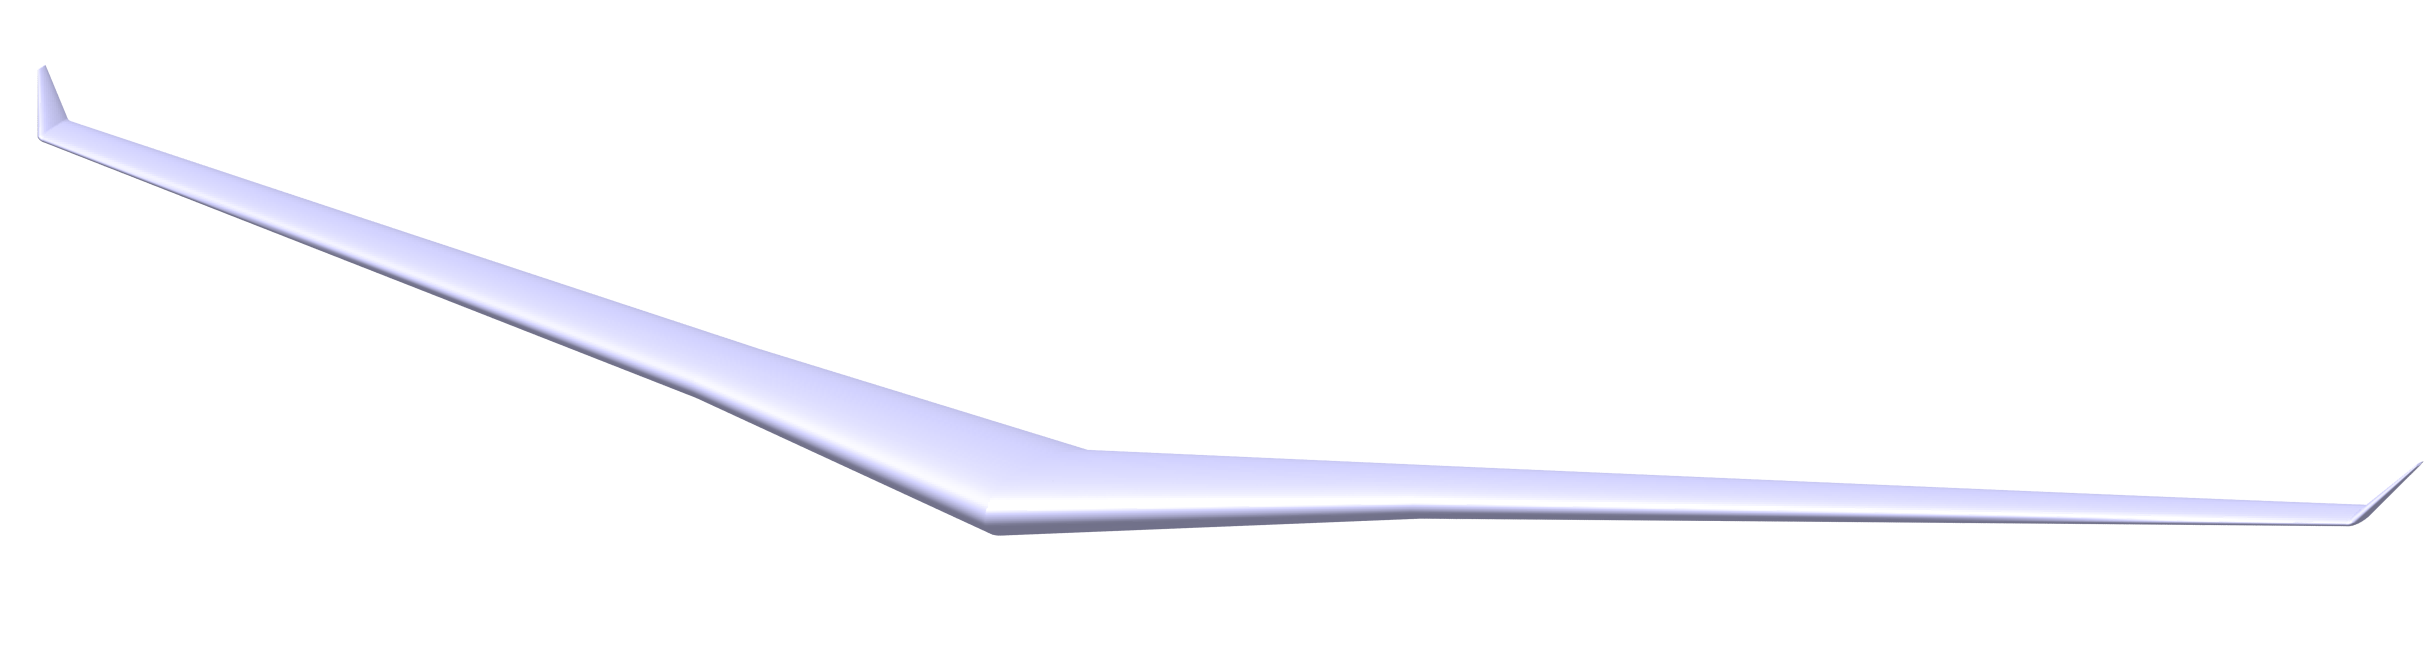
\includegraphics[width= \textwidth ]{images/fileImg/Parte_3-Aerodinamica_Velivolo_A340-200/CadAlaAirbusA340-200.png}
\caption{\footnotesize \emph{Rendering} CAD ala Airbus A340-200. CATIA V5-6R2017}
\label {fig:V2}
\end {figure}

\begin {figure} [h!]
\centering
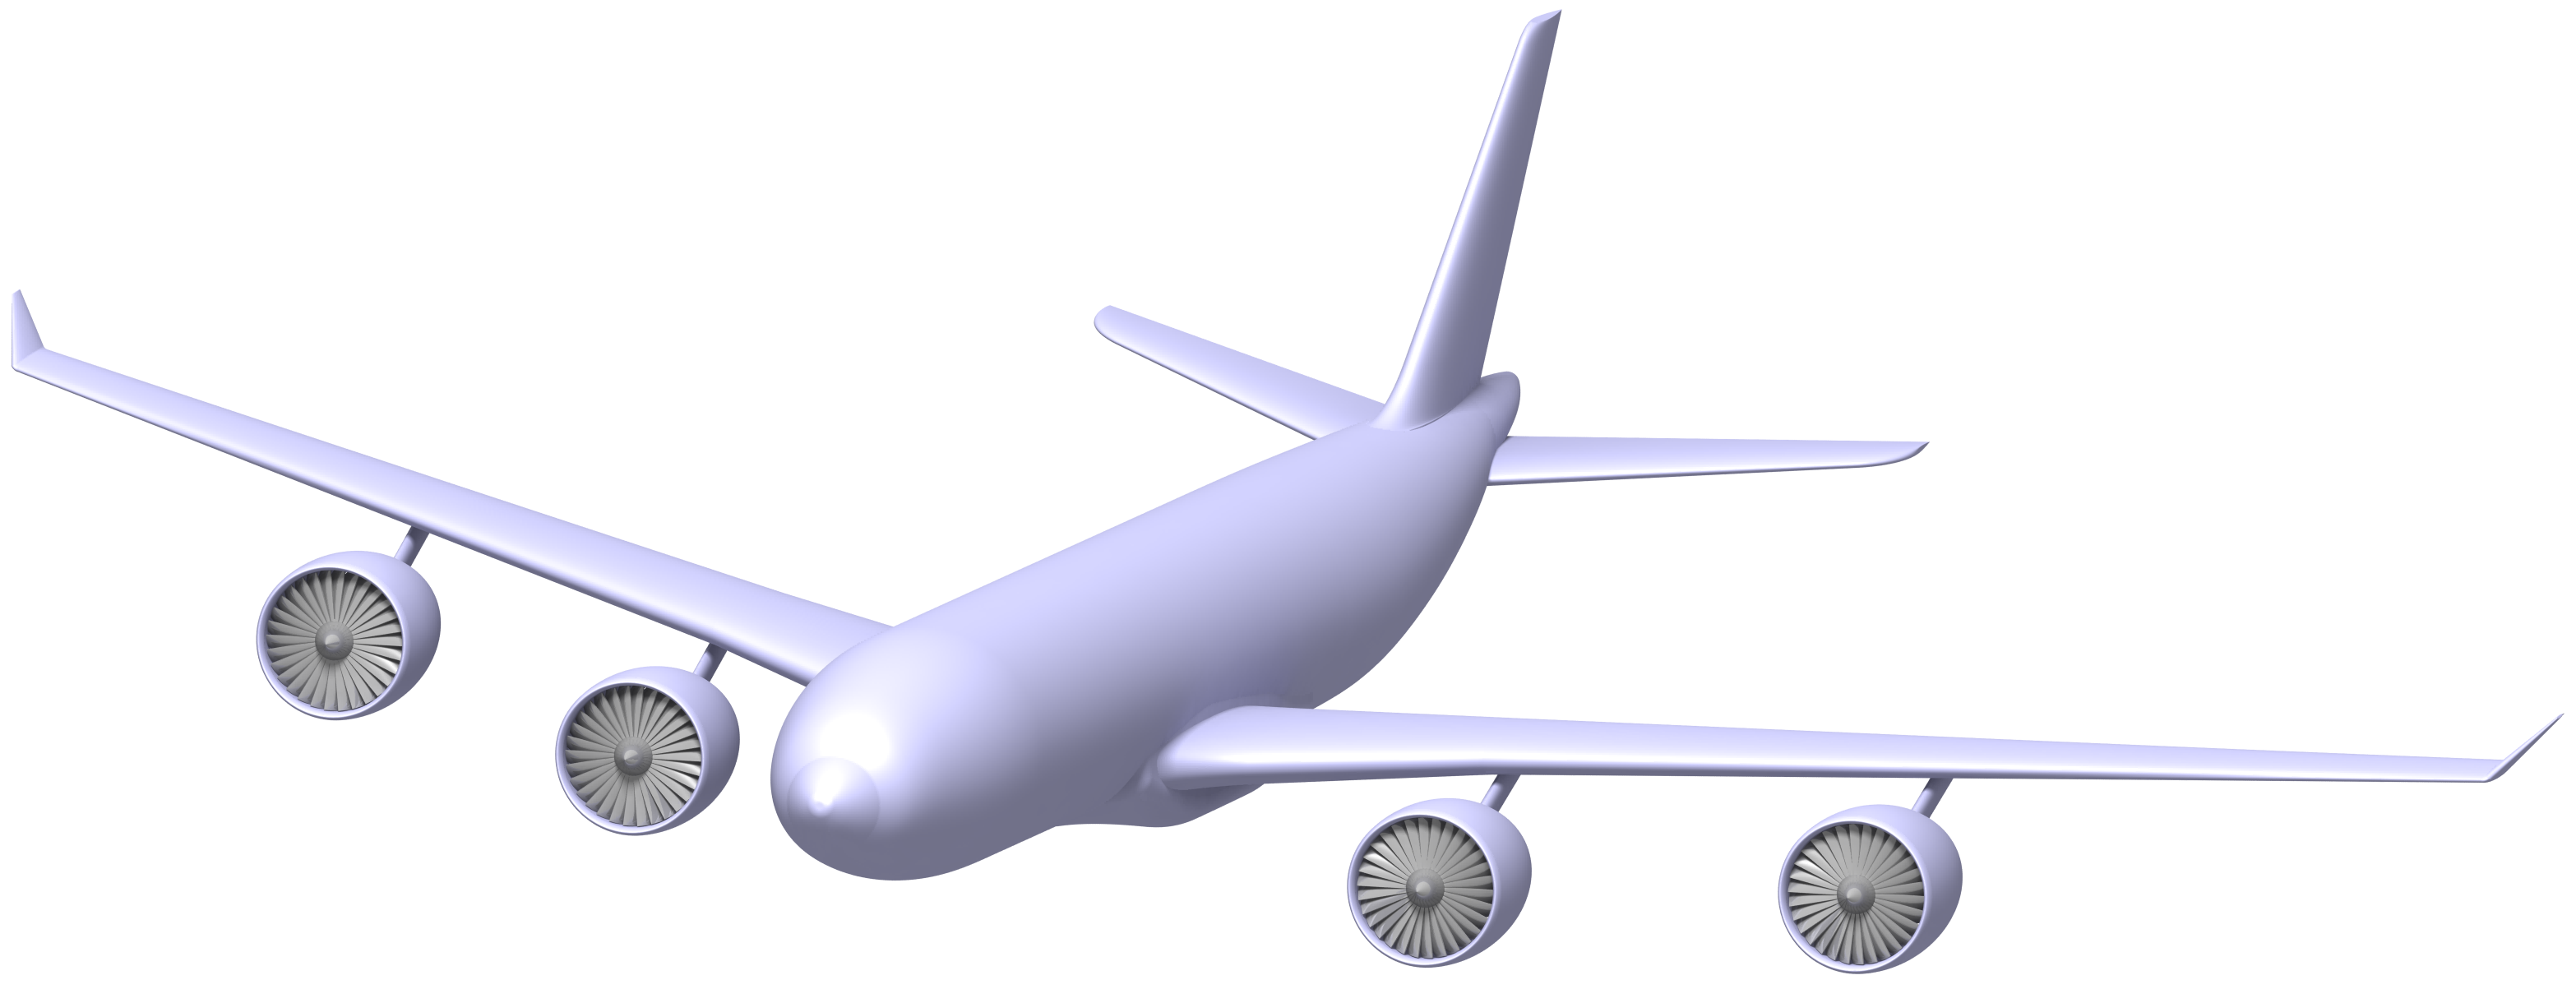
\includegraphics[width= \textwidth ]{images/fileImg/Parte_3-Aerodinamica_Velivolo_A340-200/RenderingA340-200.png}
\caption{\footnotesize \emph{Rendering} CAD velivolo Airbus A340-200. CATIA V5-6R2017}
\label {fig:V3}
\end {figure}


